\section{Classifier}\label{section:mc-cnn}
    \par{
        The ROIs are then fed into the third part of the proposed architecture, the \emph{classifier}, and properly classified as flawless or flawed; in the latter case, they are assigned a defect class.
    }
    \begin{figure}
        \centering
        \begin{tikzpicture}
            % image
            \node[circle, draw] (input) at (0,0) {I};
    
            % preprocessed image
            \node[rectangle, draw] (p1) at ($(input) + (1.5,2)$) {P};
            \node[rectangle, draw] (p2) at ($(input) + (1.5,.5)$) {P};
            \node (p3) at ($(input) + (1.5,-.5)$) {\vdots};
            \node[rectangle, draw] (p4) at ($(input) + (1.5,-2)$) {P};
    
            % image to preprocessed image
            \draw[->] ($(input) + (0.5, 0)$) -- ($(p1) + (-0.3, 0)$);
            \draw[->] ($(input) + (0.5, 0)$) -- ($(p2) + (-0.3, 0)$);
            \draw[->] ($(input) + (0.5, 0)$) -- ($(p4) + (-0.3, 0)$);
    
            % cnn
            \node[rounded rectangle, draw, minimum width=2.5cm, minimum height=1cm] (cnn1) at ($(p1) + (2,0)$) {CNN};
            \node[rounded rectangle, draw, minimum width=2.5cm, minimum height=1cm] (cnn2) at ($(p2) + (2,0)$) {CNN};
            \node[minimum width=2.5cm, minimum height=1cm] (cnn3) at ($(p3) + (2,0)$) {\vdots};
            \node[rounded rectangle, draw, minimum width=2.5cm, minimum height=1cm] (cnn4) at ($(p4) + (2,0)$) {CNN};
    
            % preprocessed to cnn
            \draw[->] ($(p1) + (0.5, 0)$) -- ($(cnn1) + (-1.2, 0)$);
            \draw[->] ($(p2) + (0.5, 0)$) -- ($(cnn2) + (-1.2, 0)$);
            \draw[->] ($(p4) + (0.5, 0)$) -- ($(cnn4) + (-1.2, 0)$);
    
            % classifier
            \node[rounded rectangle, draw] (classifier) at ($(cnn3) + (2.5,0.5)$) {NN};
    
            % cnn to classifier
            \draw[->] ($(cnn1) + (1.3, 0)$) -- ($(classifier) + (-.5, .2)$);
            \draw[->] ($(cnn2) + (1.3, 0)$) -- ($(classifier) + (-.5, 0)$);
            \draw[->] ($(cnn4) + (1.3, 0)$) -- ($(classifier) + (-.5, -.2)$);
    
            % output
            \node[circle, draw] (output) at ($(classifier) + (1.3,0)$) {O};
    
            % classifier to output
            \draw[->] ($(classifier) + (.5, 0)$) -- ($(output) + (-.45, 0)$);
    
        \end{tikzpicture}
        \caption{General structure of a MC-CNN.}\label{fig:mc-cnn}
    \end{figure}
    \par{
        The \emph{classifier} is structured as a MC-CNN, which in general has the structure illustrated in \emph{Figure \ref{fig:mc-cnn}}. 
    }
    \par{
        Firstly, the input image I is preprocessed to extract $n$ column input P.
    }
    \par{
        Secondly, these P are fed into different CNNs in parallel, therefore all the columns are independent one another. 
    }
    \par{
        Finally, the output of the MC-CNN columns is combined through a classifier, e.g. a neural network (NN), to produce the final output.
    }
    \par{
        The choice of using a MC-CNN is due to several reasons, beyond the proved effectiveness described in \cite{ieee:6248110}.
    }
    \par{
        Primarily, the training of a MC-CNN is highly parallelizable, indeed the different columns can learn separately one from another, once their correspective input is prepared.
    }
    \par{
        Moreover, it is possible to merge both local and global information in a far easier way then using a traditional, single-column, CNN. Indeed, instead of focusing only on a rectangular area, which brings only the local information about the plausible defect, with a MC-CNN it is immediate to add another column concerned with the whole image.
    }
    \par{
        This is the main point in favour of MC-CNN, since the class of a defect may be inferred using global patterns, such as the number of similar area. Imagine, for example, an error burst on the surface. Although traditional single-column CNNs may consider directly the input to the global column, this would face problems regarding the presence of multiple defects classes on the same surface. Therefore, a MC-CNN approach with some columns concerning local information and other focusing on global patterns is heuristically better.
    }
    \par{
        In \emph{Section \ref{section:further-work}} another approach to combine such information through a CNN is described. Although possible, is patently more convoluted then the MC-CNN approach. It would still be interesting to compare them in order to better evaluate the effectiveness of the proposed architecture. 
    }
    \par{
        Observe that the output of the global column must be calculated only once per each image, since it is constant throughtout the single surface, hence both the training and the predicting process can be lighten.
    }
    \par{
        Finally, as an incidental outcome, it is possible to further study the amount of contribution of the different columns in accurately determining the defective class, if any, of the considered area. These considerations are reported in \emph{Section \ref{section:results}}.
    }
    \par{
        The proposed MC-CNN has three columns, namely a \emph{shape}, a \emph{local} and a \emph{global} column.
    }
    \par{
        A final consideration about the architecture training has to be done in order to comprehend the upper bound reported in \emph{Section \ref{section:results}}. Indeed, the \emph{classifier} was implemented before the \emph{detector}. In fact, although the former relies on the latter for the ROIs and their relative features (described in \emph{Section \ref{section:shape-column}}, \emph{\ref{section:local-column}} and \emph{\ref{section:global-column}}), it was preempting supposed to have an ideal \emph{detector}, i.e. one which proposes the optimal ROIs.
    }
    \par{
        This effort-outcome oriented approach was done for two main reasons.
    }
    \par{
        Firstly, it highlights the upper bound reachable with the whole architecture.
    }
    \par{
        Secondly, dividing the \emph{detector} outcome from the \emph{classifier} input during the training allows to export the trained MC-CNN and to use it within the challenger architecture, proposed in \emph{Section \ref{section:further-work}}.
    }
    \par{
        All the three columns share the common ideas used in edge-cutting work \cite{stanford:cs231n} in their structure, beside some their idiosyncrasies. These are explained in \emph{Section \ref{section:shape-column}}, \emph{\ref{section:local-column}} and \emph{\ref{section:global-column}}.
    }
    \par{
        The basic principles used in structuring the CNNs are mainly three:
        \begin{enumerate}
            \item The input layer should be a multiple of a high power of $2$. Common dimensions are $32$ (e.g. CIFAR-10), $64$, $96$ (e.g. STL-10), or $224$ (e.g. common ImageNet ConvNets), $384$, and $512$. However, the approach described in this paper deals with input images of various size.
            \item The convolutional layers should involve small filters (e.g. $3\times 3$ or $5\times5$), using a unitary stride, should not alter the spatial dimensions of the input. Hence, proper padding (e.g., $\left[1,1,1,1\right]$ for $3\times 3$ filters) should be added.
            \item The reduction of the size of the input should be due to the pooling layers, tipically a $2\times 2$ downsampling with a $2\times 2$ stride. This is also connected with the usual constraint on input size.
        \end{enumerate}
    }
    \subsection{Shape column}\label{section:shape-column}
        \par{
            The \emph{shape column} is concerned to learn from the shape of the proposed region. This is fed into the CNN as a binary matrix, in which ones represent points in the border of the area.
        }
        \begin{figure}
            \centering
            \includegraphics[width=\linewidth]{graphics/architecture/mc-cnn-shape}
            \vskip 0.05cm
            \includegraphics[width=\linewidth]{graphics/architecture/mc-cnn-shape-filled}
            \caption{Shape column input (top) and input filled (bottom).}\label{fig:mc-cnn:shape-input}
        \end{figure}
        \par{
            An example of this binary images is given in \emph{Figure \ref{fig:mc-cnn:shape-input}} (top). The shape is centered in a $1600\times 256$ black image. Indeed, the size of the input is set to the largest area that could be found, i.e. a defect spanning over the entire surface. The shape is centered to ensure that the classifier is translation independent. 
        }
        \par{
            The \emph{detector}, since is not ideal, provides to the \emph{classifier} also false positive ROIs, i.e. regions that are not defective. Therefore, this stage of the architecture need to be able to discard flawless proposed regions.
        }
        \par{
            However, training the shape column to classify some shapes as not defective is not feasible. Indeed, there is not a flawless surface shape, and manually generating it would not be safe.
        }
        \par{
            Hence, the shape column should only be trained to classify a region into one of the four defect classes, and to mark flawless proposals will be duty of the final classifier (\emph{Section \ref{section:final-classifier}}).
        }
        \par{
            Therefore, the output layer is a $n$-dimensional vector, where $n$ is the number of defect classes. Each entry of this vector describes the confidence of the network in considering the input shape as related to one of the $n$ defect classes.
        }
        \par{
            However, from data analysis was observed that sometimes defective input defects of the same class are clustered together, since very near one another. This is usually true for defects of class No.3, which are burst defects and might be nearly adjacent. Therefore, the shape that would be extracted is the shape of the region and not the one of the defects. Hence, the network would not be properly trained.
        }
        \par{
            For this reason, the shape column is left as a further development in \emph{Section \ref{section:further-work}}.
        }
        \par{
            The shape column input could also be filled before to be fed into the CNN, as shown in \emph{Figure \ref{fig:mc-cnn:shape-input}} (bottom).
        }
    \subsection{Local column}\label{section:local-column}
        \par{
            The \emph{local column} is thought to consider luminance levels around the border of the defect, to learn from the local context. Similarly to the shape column (\emph{Section \ref{section:shape-column}}), this column is concerned only in classifying proposals into one of the four defective classes.
        }
        \begin{figure}
            \centering
            \includegraphics[width=\linewidth]{graphics/architecture/mc-cnn-local}
            \caption{Local column input.}\label{fig:mc-cnn:local-input}
        \end{figure}
        \par{
            Therefore, the column is fed with the grey scale portion of the image inside the bounding box of the considered region. As an example, in \emph{Figure \ref{fig:mc-cnn:local-input}} is illustrated a plausible input to the \emph{local column}.
        }
        \par{
            This grey scale portion is generated from the shape of the region and the original image.
        }
        \par{
            Firstly, the bounding box of the shape is calculated. Secondly, the original image outside the bounding box is discarded. Finally, the cropped image is centered in a black $1600\times 256$ picture. The reasons behind the centering and the dimensioning of the input are the same described in \emph{Section \ref{section:shape-column}}.
        }
        \begin{table*}
            \centering
            \normalsize
            \begin{tabular}{|l|l|l|l|}
                \hline
                    \textbf{Layer} & \textbf{Type} & \textbf{Activations} & \textbf{Learnables}\\\hline
                    Input & Image input & $256\times 1600 \times 1 = 409.600$ & \\
                    $\left[256\times 1600\times 1\right]$ image & & & \\
                    ``zerocenter'' normalization & & & \\\hline
                    %%%%
                    Spreader & Convolution & $800\times 800\times 4 = 2.560.000$ & Weights $3\times 3\times 1 \times 4 = 36$\\
                    Filter $4$ $\left[3\times 3\times 1\right]$ & & & Bias $1\times 1\times 4 = 4$\\
                    Stride $\left[1\;1\right]$ & & & Total: $40$ \\
                    Dilation factor $\left[400\;400\right]$ & & & \\
                    Padding $\left[672\;0\right]$ & & & \\\hline
                    %%%%
                    Conv1 & Convolution & $800\times 800\times 8 = 5.120.000$ & Weights $3\times 3\times 4 \times 8 = 288$\\
                    Filter $8$ $\left[3\times 3\times 1\right]$ & & & Bias $1\times 1\times 8 = 8$\\
                    Stride $\left[1\;1\right]$ & & & Total: $296$\\
                    Padding ``same'' & & & \\\hline
                    %%%%
                    MaxPool1, $\left[4\times 4\times 1\right]$ & Max pooling & $200\times 200\times 8 = 320.000$ & \\
                    Stride $\left[4\;4\right]$ & & & \\
                    Padding ``same'' & & & \\\hline
                    %%%%
                    Conv2 & Convolution & $200\times 200\times 16 = 640.000$ & Weights $3\times 3\times 8 \times 16 = 1152$\\
                    Filter $16$ $\left[3\times 3\times 1\right]$ & & & Bias $1\times 1\times 16 = 16$\\
                    Stride $\left[1\;1\right]$ & & & Total: $1168$\\
                    Padding ``same'' & & & \\\hline
                    %%%%
                    MaxPool2, $\left[4\times 4\times 1\right]$ & Max pooling & $50\times 50\times 16 = 40.000$ & \\
                    Stride $\left[4\;4\right]$ & & & \\
                    Padding ``same'' & & & \\\hline
                    %%%%
                    Conv3 & Convolution & $50\times 50\times 32 = 640.000$ & Weights $3\times 3\times 16 \times 32 = 4.608$\\
                    Filter $32$ $\left[3\times 3\times 1\right]$ & & & Bias $1\times 1\times 32 = 32$\\
                    Stride $\left[1\;1\right]$ & & & Total: $4640$\\
                    Padding ``same'' & & & \\\hline
                    %%%%
                    MaxPool3, $\left[2\times 2\times 1\right]$& Max pooling & $25\times 25\times 32 = 20.000$ & \\
                    Stride $\left[2\;2\right]$ & & & \\
                    Padding ``same'' & & & \\\hline
                    %%%%
                    Conv4 & Convolution & $25\times 25\times 64 = 40.000$ & Weights $3\times 3\times 32 \times 64 = 18.432$\\
                    Filter $64$ $\left[3\times 3\times 1\right]$ & & & Bias $1\times 1\times 64 = 64$\\
                    Stride $\left[1\;1\right]$ & & & Total: $18496$\\
                    Padding ``same'' & & & \\\hline
                    %%%%
                    MaxPool4, $\left[2\times 2\times 1\right]$ & Max pooling & $13\times 13\times 64 = 10.816$ & \\
                    Stride $\left[2\;2\right]$ & & & \\
                    Padding ``same'' & & & \\\hline
                    %%%%
                    Conv5 & Convolution & $13\times 13\times 128 = 21.632$ & Weights $3\times 3\times 64 \times 128 = 73.728$\\
                    Filter $128$ $\left[3\times 3\times 1\right]$ & & & Bias $1\times 1\times 128 = 128$\\
                    Stride $\left[1\;1\right]$ & & & Total: $73856$\\
                    Padding ``same'' & & & \\\hline
                    %%%%
                    MaxPool5, $\left[2\times 2\times 1\right]$ & Max pooling & $7\times 7\times 128 = 6.272$ & \\
                    Stride $\left[2\;2\right]$ & & & \\
                    Padding ``same'' & & & \\\hline
                    %%%%
                    FullConn1 & Fully connected & $1\times 1\times 16 = 16$ & Weights $16\times 6272 = 100.352$\\
                    & & & Bias $16\times 1 = 16$\\
                    & & & Total: $100.368$\\\hline
                    %%%%
                    FullConn2 & Fully connected & $1\times 1\times 16 = 16$ & Weights $16\times 16 = 256$\\
                    & & & Bias $16\times 1 = 16$\\
                    & & & Total: $272$\\\hline
                    %%%%
                    FullConn3 & Fully connected & $1\times 1\times 4 = 4$ & Weights $4\times 16 = 64$\\
                    & & & Bias $4\times 1 = 4$\\
                    & & & Total: $68$\\\hline
                    %%%%
                    Output & Softmax & $1\times 1\times 4 = 4$ & \\
                \hline
            \end{tabular}
            \vspace{0.5cm}
            \caption{Local column CNN layers.}\label{table:mc-cnn:local-structure}
        \end{table*}
        \par{
            The layers of this CNN are shown in \emph{Table \ref{table:mc-cnn:local-structure}}.
        }
        \par{
            The output layer is analogous to the one in \emph{Section \ref{section:shape-column}}.
        }
        \par{
            The peculiarity of this CNN lies in its first convolutional layer, named \emph{spreader}. It is a novel application of the dilation factor. 
        }
        \par{
            Recall that given a $n\times n$ filter, a dilation of $[a\;b]$ applied to the given filter produces a $\left[\left(n-1\right)*a + 1\right] \times \left[\left(n-1\right)*b + 1\right]$ filter. The original entries are equally spread in the new filter, whereas the additional values are null.
        }
        \par{
            As an example, the below transformation applies a dilation factor of $\left[3\;5\right]$ to the given $2\times 2$ filter.
        }
        \begin{BVerbatim}
            
                          _           _
     _   _               | a 0 0 0 0 b |
    | a b |   [3 5]      | 0 0 0 0 0 0 |
    | c d |  ------>     | 0 0 0 0 0 0 |
     -   -               | c 0 0 0 0 d |
                          -           -
                    
        \end{BVerbatim}
        \par{
            An example on a $3\times 3$ filter is proposed below:
        } 
        \begin{BVerbatim}
            
                            _         _
     _     _               | a 0 b 0 c |
    | a b c |   [2 2]      | 0 0 0 0 0 |
    | d e f |  ------>     | d 0 e 0 f |
    | g h i |              | 0 0 0 0 0 |
     -     -               | g 0 h 0 i |
                            -         -
                    
        \end{BVerbatim}
        \par{
            The dilation factor is used in CNNs to implement a wider receptive field, using the same number of weights. Indeed, a $K_1 \times K_2$ filter convolves pixels in an area of $K_1 \times K_2$. Using a dilation factor of $\left[a\;b\right]$ it would convolve the same number of pixels, but on an area of $\left[\left(K_1-1\right)*a + 1\right] \times \left[\left(K_2-1\right)*b + 1\right]$. Using a proper stride, this would be the same of a downsampling followed by a convolution.
        }
        \par{
            However, in the proposed architecture it is used in a novel way, to address the problem of different-sized bounding boxes.
        }
        \par{
            In fact, the usage of the \emph{spreader} layer aims to reproduce in different location of the activation the original informative regions, through some learned linear functions. Indeed, with a proper sizing, the convolution in the first layer results in the sum of the bias factor and a single informative pixel multiplied by a weight of the filter.
        }
        \begin{figure}
            \centering
            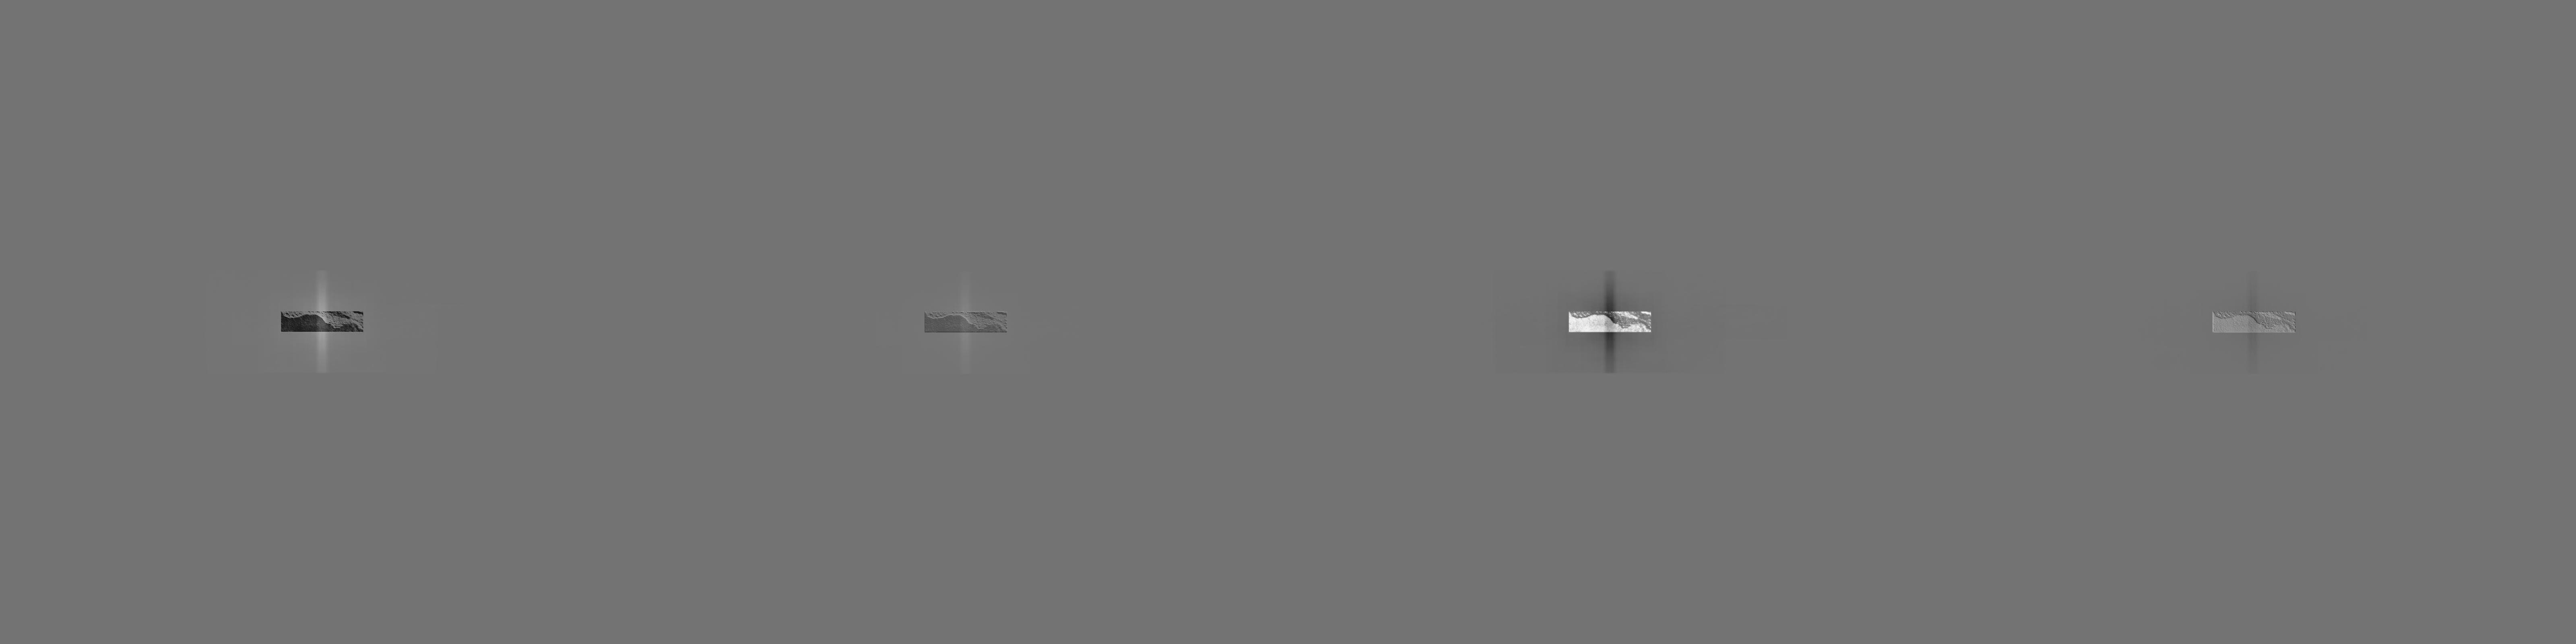
\includegraphics[width=\linewidth]{graphics/architecture/act_net}
            \vskip .05cm
            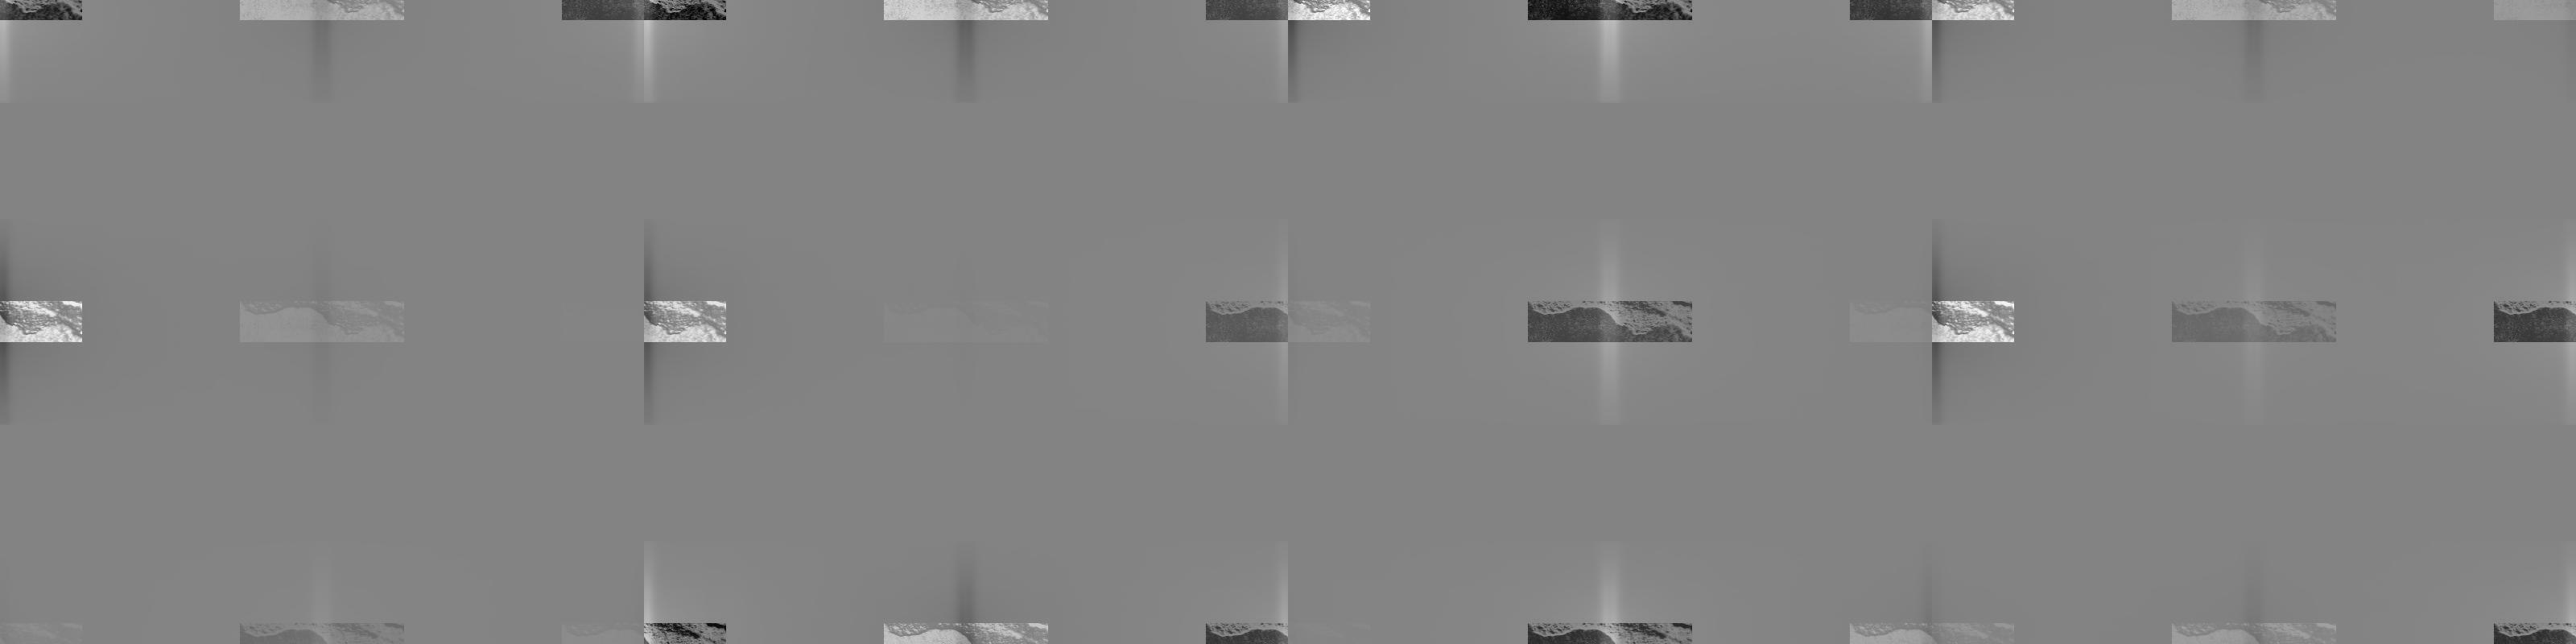
\includegraphics[width=\linewidth]{graphics/architecture/act_net_hope}
            \caption{Learned features with a traditional convolutional layer (top) and with the \emph{spreader} (bottom). $4$ tiled features are illustrated in both cases.}\label{fig:learned-features-hope-net}
        \end{figure}
        \par{
            In \emph{Figure \ref{fig:learned-features-hope-net}} the learned features of four $3\times3$ filters of a traditional convolutional layer with padding $\left[673\;1\right]$ are juxtaposed to the ones learned by four $3\times 3$ filters with a dilation factor of $\left[400\;400\right]$ and proper padding $\left[672\;0\right]$. 
        }
        \par{
            The two pictures are scaled to be paired. However, the former is $1600 \times 1600$, the latter is $800\times 800$. Still it is patent that the proposed approach greatly exceed the traditional one in terms of information kept. 
        }
        \par{
            Indeed, the problem with convolutional layer with massive padding (in alternative to cropping) is that large empty regions have null activations. Then, pooling layers keep the proportions between \emph{death} area and the informative, central, region. This leads to a lot of memory waste.
        }
        \par{
            A $3\times 3$ filter with a dilation factor of half the output activation size and proper padding enhance the effectiveness of following layers, recycling empty areas. In fact, they are convolved with the central informative region.
        }
        \par{
            Indeed, this approach ensures that at least $9$ areas will convolve with the defective region. The learned weights of the filter will then decide whether to copy, along with some multiplicative factor (which can be thought as varying the exposure of the image portion), the defect in these new regions.
        }
        \par{
            It would eventually learn to handle large original pictures. As an example, if the dataset is composed by a cornucopia of large defects, the \emph{spreader} could copy only vertically the defect, using only three of the nine available weights.
        }
        \par{
            In the proposed architecture, four of this spreading filters are used in the first layer, conceptually in order to tune them one per defect class.
        }
        \par{
            The \emph{spreader} layer represents an effective alternative to either lossy crop or padding when dealing with either images of different dimensions or non-squared pictures.
        }
        \par{
            By cropping the image, massive memory saving could be allowed. As an example, the $512\times 512$ cropping proposed in \emph{Table \ref{table:cropping}} would save $800\times 800 - 512\times 512 \approx \SI{1}{\mega\byte}$ per image, about $59.04\%$.
        }
        \par{
            However, the proposed spreader introduces $\times 9$ information compared to cropping, which is followed by activations similar, although with less memory consumption, to the ones shown in \emph{Figure \ref{fig:learned-features-hope-net}} (top).
        }
        \par{
            There is patently a tradeoff between training time, memory (hence both batch and mini-bath size), number of weights and information loss.
        }
        \par{
            Using a classical approach with these different-sized bounding boxes, with either cropping or padding, would conceptually lead at the end to suppress informative areas, due both to pooling and convolving empty regions.
        }
        \begin{figure}
            \centering
            \begin{subfigure}{.5\linewidth}
                \centering
                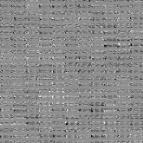
\includegraphics[width=.9\linewidth]{graphics/architecture/act_net_out}
                % \caption{}
            \end{subfigure}\hfill
            \begin{subfigure}{.5\linewidth}
                \centering
                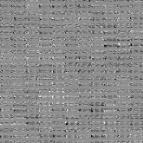
\includegraphics[width=.9\linewidth]{graphics/architecture/act_net_hope_out}
                % \caption{}
            \end{subfigure}
            \caption{Final layer features with classical architecture ($512$ $13\times 13$ features) (a) and with the \emph{spreader} ($128$ $13\times 13$ features) (b).}
            \label{fig:features-last-layer}
        \end{figure}
        \par{
            Instead, the proposed initial layer spreads over the squared activation matrix the defect, allowing in the final layer to have more informative features, as visible in the comparison in \emph{Figure \ref{fig:features-last-layer}}. Indeed, the visual effect of equivalence between the two suggests that the initial \emph{spreader} reduces the number of successive filters required, hence the number of parameters. 
        }
        \par{
            A smaller number of parameters requires less data to prevent overfitting. If the outcomes are the same, it means that the model is better.
        }
        \par{
            What can be heuristically inferred is that what is lost as memory efficiency, is far more gained as information. Hence, the memory can be saved in successive layers of the architecture. In the proposed architecture this has be done through the first two max pooling layers, each of them introducing a shrinking factor of $4$.
        }
        \par{
            Moreover, performing a massive crop operation one accepts to misclassify a given percentage of the dataset. From an intuitive point of view, the \emph{spreader} could learn to repeat the defect only vertically.
            For example, the filter:
        }
        \par{
        \begin{BVerbatim}

            _     _
           | 1 0 0 |
           | 1 0 0 |
           | 1 0 0 |
            -     -
       \end{BVerbatim}
        }
        \par{
            would simply replicate three times the image vertically. The takeaway is that this filter removes the manual tuning of the crop operation, while it improves the efficiency of the feature extraction stage of the CNN.
        }
        \par{
            However, evaluating the results of the crop operation is proposed as further development in \emph{Section \ref{section:further-work}}.
        }
    \subsection{Global column}\label{section:global-column}
        \begin{figure}
            \centering
            \includegraphics[width=\linewidth]{graphics/architecture/mc-cnn-global}
            \caption{Global column input.}\label{fig:mc-cnn:global-input}
        \end{figure}
        \par{
            The \emph{global column} is concerned in detecting global patterns, like zipper cracks. Hence, it is fed with the whole image. An example of input is shown in \emph{Figure \ref{fig:mc-cnn:global-input}}. The importance of this column is clear from the observations made in \emph{Section \ref{subsection:defects}}. Indeed, when two different classes are locally equal, the global column is determinant to correctly classify the defects.
        }
        \par{
            Ideally, the global column should output a $16$-dimensional vector, with one entry per combination of classes. The presence of at least a defect of a particular class is hot-encoded in a $4$-bit bitmask.
        }
        \par{
            However, the dataset is very skewed when accounting for different classes combinations, as illustrated in \emph{Figure \ref{fig:defects:combinations}}. Hence, the output layer has to be structured in a different way. Moreover, the inner structure of the CNN has to be deeper and requires a larger amount of data and 
            , therefore, longer training times and more hardware resources then the local column.
        }
        \par{
            Therefore, the global column is left as a further development in \emph{Section \ref{section:further-work}}.
        }
    \subsection{Final classifier}\label{section:final-classifier}
        \par{
            The outcomes of the different columns of a MC-CNN are then combined to obtain the final output. In the proposed architecture, this combination is done through a neural network, since a manual tuning of such combination would be ineffective. Moreover, this is used to establish thresholding.
        }
        \begin{figure}
            \centering
            \begin{tikzpicture}
                % input layer
                \foreach \i in {0,...,23}
                    \node[circle, draw, minimum height=1, minimum width=1,fill=blue] (input \i) at (0,-\i*0.5) {};

                % hidden layer
                \foreach \i in {0,...,15}
                    \node[circle, draw, minimum height=1, minimum width=1,fill=orange] (hidden \i) at ($(input 4) + (2,-\i*0.5)$) {};

                % from input to hidden layer
                \foreach \i in {0,...,23}
                    \foreach \j in {0,...,15}
                        \draw ($(input \i) + (.2,0)$) -- ($(hidden \j) + (-.2,0)$);

                % hidden layer 2
                \foreach \i in {0,...,15}
                    \node[circle, draw, minimum height=1, minimum width=1,fill=orange] (hidden 2 \i) at ($(hidden 0) + (2,-\i*0.5)$) {};

                % from hidden to hidden layer
                \foreach \i in {0,...,15}
                    \foreach \j in {0,...,15}
                        \draw ($(hidden \i) + (.2,0)$) -- ($(hidden 2 \j) + (-.2,0)$);

                % output layer
                \foreach \i in {0,...,4}
                    \node[circle, draw, minimum height=1, minimum width=1,fill=yellow] (output \i) at ($(hidden 2 5) + (2,-\i*0.5)$) {};

                % from hidden 2 to output layer
                \foreach \i in {0,...,15}
                    \foreach \j in {0,...,4}
                        \draw ($(hidden 2 \i) + (.2,0)$) -- ($(output \j) + (-.2,0)$);

                % from output to softmax layer
                \foreach \i in {0,...,4}
                    \draw ($(output \i) + (.2,0)$) -- ($(output \i) + (2,0)$);

                % softmax layer
                \node[rounded rectangle, fill=white, minimum width=3cm,draw,rotate=-90] (softmax) at ($(output 2) + (1,0)$) {Softmax};

                % legend
                \node[rectangle, draw, fill=yellow, minimum width=1, minimum height=1] (output label color) at ($(output 0) + (0,1)$) {};
                \node[anchor=west] (output label) at ($(output label color) + (.2,0)$) {Output layer};

                \node[rectangle, draw, fill=orange, minimum width=1, minimum height=1] (hidden label color) at ($(output label color) + (0,.5)$) {};
                \node[anchor=west] (hidden label) at ($(hidden label color) + (.2,0)$) {Hidden layer};

                \node[rectangle, draw, fill=blue, minimum width=1, minimum height=1] (input label color) at ($(hidden label color) + (0,.5)$) {};
                \node[anchor=west] (input label) at ($(input label color) + (.2,0)$) {Input layer};

                \node[anchor=west] (legend label) at ($(input label color) + (-.25,.5)$) {\underline{Legend}};
            \end{tikzpicture}
            \caption{Final classifier structure.}\label{fig:mc-cnn:final-classifier-structure}
        \end{figure}
        \par{
            In \emph{Figure \ref{fig:mc-cnn:final-classifier-structure}} the structure of the last layer of the architecture is described.
        }
        \par{
            The first layer is constrained to the output size of the three columns, i.e. $4+4+16 = 24$. Then there are two hidden layers with $16$ activation units, and finally the output layer with $5$ neurons. The output is passed through a softmax layer, hence the final output describe the confidence per each class.
        }
        \par{
            Observe that bias units have not been included in the picture.
        }
        \par{
            The classifier is left as further work, together with both shape and global columns, in \emph{Section \ref{section:further-work}}.
        }
